\documentclass[sigconf]{acmart}
\usepackage{booktabs}
\usepackage{multirow} % Add this to your LaTeX preamble
\usepackage{subfigure} % For arranging images
\usepackage{graphicx}  % For including images
\usepackage{tcolorbox} % For colored background

%% \BibTeX command to typeset BibTeX logo in the docs
\AtBeginDocument{%
  \providecommand\BibTeX{{%
    \normalfont B\kern-0.5em{\scshape i\kern-0.25em b}\kern-0.8em\TeX}}}

%% These commands are for a PROCEEDINGS abstract or paper.
\settopmatter{printacmref=false} % Removes citation information below abstract
\renewcommand\footnotetextcopyrightpermission[1]{} % removes footnote with conference information in 

\acmConference[AEPRO 2025]{AEPRO 2025: Algorithm Engineering Projects}{March 1}{Jena, Germany}

% convert text to title case
% http://individed.com/code/to-title-case/

% that helps you to formulate your sentences
% https://www.deepl.com/translator

\begin{document}

%%
%% The "title" command has an optional parameter,
%% allowing the author to define a "short title" to be used in page headers.
\title[Parallelized and Vectorized Image Enhancing Algorithm for Scanning or Printing]{Parallelized and Vectorized Image Enhancing Algorithm for Scanning or Printing \\\large Algorithm Engineering 2025 Project Paper}

%%
%% The "author" command and its associated commands are used to define
%% the authors and their affiliations.

\author{Angelo Wieden}
\affiliation{%
  \institution{Friedrich Schiller University Jena}
  \country{Germany}}
\email{angelo.wieden@uni-jena.de}


%% The abstract is a short summary of the work to be presented in the article.
\begin{abstract}


This paper deals with the development of a fast, platform-independent program for image enhancement based on local pixel data. The output produces a clean black and white version of the input picture, which results in the appearance of a scanned image. This research paper aims to answer the following question. How can such an algorithm be efficiently implemented in C++, and which computational parameters could be manually tweaked on a picture-by-picture basis, for best results? The implementation of the image enhancement algorithm was done in C++, using OpenMP to parallelize and vectorize specific sections. Bataineh's binarization algorithm served as a foundation a, which was built upon. CMake was used to build and package the software. Testing was done with the help of Catch2. The standalone stb library helped in reading and writing certain image file types. The parallelized version achieves speedups of up to \texttt{12x} over the serial version. These findings demonstrate the importance of writing efficient code for modern multicore CPUs, in the area of image processing.



\end{abstract}

%%
%% Keywords. The author(s) should pick words that accurately describe
%% the work being presented. Separate the keywords with commas.
\keywords{image enhancing, algorithm engineering, parallelization, vectorization}


%%
%% This command processes the author and affiliation and title
%% information and builds the first part of the formatted document.
\maketitle

\let\thefootnote\relax\footnotetext{AEPRO 2025, March 1, Jena, Germany. Copyright \copyright 2025 for this paper by its authors. Use permitted under Creative Commons License Attribution 4.0 International (CC BY 4.0).}


\section{Introduction}

\sloppy
\subsection{Background}
Image enhancement is a broad field of digital image processing that covers a variety of tasks. Although it is mainly used to make images more readable for humans, image enhancement also finds various applications in other areas such as preprocessing for OCR or medical imaging. Traditionally, image enhancement is done serially, wasting a large amount of computational power of modern multicore CPUs. An already existing image enhancing algorithm was modified within the scope of the 2025 Algorithm Engineering Project, using full advantage of SIMD vectorization and parallelization through OpenMP for large performance gains. This particular algorithm uses binarization as a form of enhancement, which is the process of turning pixels either fully white or black depending on different factors.

\subsection{Related Work}
The algorithm that was implemented and built upon was designed on the basis of the adaptive threshold calculation used for pixel binarization by Bataineh \cite{Bataineh2011}. A different binarization approach is taken by Bradley \cite{Bradley2007}, which will be compared to mine in section 3.

\subsection{Our Contributions}
Aside from the implementation of the algorithm itself in C++, there were other means necessary like input parsing, output handling, implementing various argument flags for manual parameter tweaking and benchmarking, as well as a lot of fine-tuning, writing unit tests with Catch2 and making the program as portable as possible with the help of CMake.

\subsection{Outline}
In the following section of this paper, an explanation on how the algorithm decides which pixels should be assigned which color will be provided, as well as information on how input files are parsed, and output is handled. Furthermore, the modifications that were done to the algorithm by Bataineh will be explained. \cite{Bataineh2011}.

Section 3 shows the before-and-after experiments of enhanced documents by the proposed program. Also, there will be a comparison of our implementation and the original algorithm. At last, a performance benchmark will show the resulting speedup of the serialized and optimized versions of the algorithm on two different modern systems.

In section 4, the reader will have a look at a discussion of findings stemming from this project, and an analysis about future directions.

\section{The Algorithm}
This section explains the inner workings of the program.

\subsection{Processing of Input- and Output Files}
\label{sub:sec:preprocessing}
Upon receiving an input file, parsing happens dependent on the input file's type. The stb library handles both .jpg and .png files, and converts them to an array of color values, where each pixel is assigned 3 - red, green and blue - values ranging from 0 to 255.
The same formatting is done for .ppm files through a simple loop, as the file structure of .ppm allows for easy parsing. 

As a last preprocessing step before the binarization algorithm can start, the formatted pixel color values have to be mapped to a singular grayscale value by taking the average of the red, green and blue channels on a per-pixel basis.

To generate output files, the stb library is used for .jpg and .png files, while .ppm file writing was manually implemented. 

\subsection{Binarization Algorithm}
The C++ algorithm works by adaptively assigning each pixel a threshold of a color value, based on multiple factors. These factors are heavily influenced by the target's neighboring pixels within a window around the target. If the original image's grayscale value is less than this threshold, the enhanced image's target pixel will be black. Otherwise, the pixel will turn white.

To calculate the threshold value of a pixel, a series of calculations need to be done:

\begin{enumerate}
    \item \textbf{Mean Color Value of the Image:}  
    \begin{equation}
        \mu = \frac{1}{N} \sum_{i=1}^{N} I_i
    \end{equation}
    where \( \mu \) is the mean color value, \( N \) is the total number of pixels, and \( I_i \) represents the grayscale intensity of the \( i \)-th pixel.

    \item \textbf{Each Pixel's Deviation from the Mean:}  
    \begin{equation}
        D_i = | I_i - \mu |
    \end{equation}
    where \( D_i \) is the absolute deviation of pixel \( i \) from the mean.

    \item \textbf{Standard Deviation of the Image:}  
    \begin{equation}
        \sigma = \sqrt{\frac{1}{N} \sum_{i=1}^{N} (I_i - \mu)^2}
    \end{equation}
    where \( \sigma \) is the standard deviation.

    \item \textbf{Minimum and Maximum Deviation Values:}  
    \begin{equation}
        D_{\min} = \min_{i} D_i, \quad D_{\max} = \max_{i} D_i
    \end{equation}
    where \( D_{\min} \) and \( D_{\max} \) represent the minimum and maximum deviations, respectively. It should be noted that the original algorithm by Bataineh \cite{Bataineh2011} used the minimum and maximum values of all windows. Testing revealed that this approach provides similar results with reduced computational load.

    \item \textbf{Window Borders and Number of Pixels within the Window:}  
    \begin{align}
        y_{\text{start}} &= \max(0, y_i - \frac{W_\text{size}}{2}) \\
        x_{\text{start}} &= \max(0, x_i - \frac{W_\text{size}}{2}) \\
        y_{\text{end}} &= \min(y_i + \frac{W_\text{size}}{2}, h - 1) \\
        x_{\text{end}} &= \min(x_i + \frac{W_\text{size}}{2}, w - 1) \\
        N_{\text{window}} &= (x_{\text{end}} - x_{\text{start}} + 1) \times (y_{\text{end}} - y_{\text{start}} + 1)
    \end{align}
    where \( W_\text{size} \) is the window size, \( h \) and \( w \) are the image height and width, and \( N_{\text{window}} \) is the total number of pixels in the window centered at pixel \( i \).

    \item \textbf{Mean Value of Pixels in a Window:}  
    \begin{equation}
        \mu_{w} = \frac{1}{N_{\text{window}}} \sum_{j \in W} I_j
    \end{equation}
    where \( \mu_{w} \) is the mean grayscale value within the window centered at pixel \( i \), and \( W \) is the set of pixels within the window.

    \item \textbf{Standard Deviation within a Window:}  
    \begin{equation}
        \sigma_{w} = \sqrt{\frac{1}{N_{\text{window}}} \sum_{j \in W} (D_j - \mu_{w})^2}
    \end{equation}
    where \( \sigma_{w} \) is the standard deviation within the window centered at pixel \( i \).

    \item \textbf{Adaptive Deviation for Each Window:}  
    \begin{equation}
        A_i = \frac{\sigma_{w} - D_{\min}}{D_{\max} - D_{\min}}
    \end{equation}
    where \( A_i \) is the adaptive deviation for the window centered at pixel \( i \).

    \item \textbf{Finally, the threshold can be calculated as:}
    \begin{equation}
        T_i = \left( \mu_{w} - \frac{\mu_{w}^2 - \sigma_{w}}{(\mu + \sigma_{w}) \cdot (A_i + \sigma_{w})} \right) \times M
    \end{equation}
    This calculation features a noise multiplier \( M \), which is an addition to the original algorithm. 
\end{enumerate}


Upon observing that some pictures needed additional preprocessing to reduce general image noise, it was found out that multiplying the threshold values by a constant between 0 and 1 will reduce more noise, the lower the constant is. The reduced noise will also result in thinner lines though, which is why this should be set to the highest value possible that results in minimal image noise. A higher window size seems to make thin lines thicker, but also has the biggest negative impact on runtime.

These steps have been successfully parallelized and vectorized through OpenMP. All necessary variables have been aligned to 64-bit registers for optimal performance.
After calculating the threshold, the final image can be constructed based on the binarization logic above.
By default, the window size is set to 20 and the noise multiplier is set to 0.9, which should work well for most images.

\subsection{Program Flags}

Multiple flags are included to manually tinker with parameters or gain more insight on the program.
These are:

\begin{itemize}
    \item \texttt{-h} for information about program usage and flags.
    \item \texttt{-v} activates verbose mode, printing information during the algorithm process.
    \item \texttt{-b} gathers the elapsed time (excluding the input processing and output writing phases) 
    \item \texttt{-s} activates the serial mode, allowing only one thread.
    \item \texttt{-o="outputDir/outputName.filetype"} to assign the output folder and filename.
    \item \texttt{-w=INT} specifies the window size.
    \item \texttt{-n=INT} sets the noise multiplier in \% (0 to 100) -> (0 to 1).
\end{itemize}

If no flags are set, the program will use a standard configuration. 

\subsection{Build and Compilation}

For build automization, CMake was chosen for cross-platform compatibility. Detailed instructions on how to build the program are in the projects readme file. 

It is highly advised to use GNU or Clang as the compiler, as MSVC does not fully support newer OpenMP functions as of now. Full MSVC support was still added in CMake and the program itself for a flawless integration once MSVC is fully compatible with OpenMP.

The program is compiled with the following flags:
\begin{itemize}
    \item \texttt{-fopenmp -O2 -march=native -mavx -ffast-math -std=c++17} for GNU / Clang
    \item \texttt{/openmp /O2 /arch:AVX /fp:fast /std:c++17} for MSVC
\end{itemize}

\subsection{Program Usage}
To enhance an image, execute the program and pass the path to the image you would like to enhance, as well as any arguments:\\ \texttt{./main path\_to\_image <args>} \\
If the output image has too much noise or the text lines appear too thin, adjust the program flags by reducing the noise multiplier or increasing the window size until the desired look is achieved.

\subsection{Unit Tests}
The compiled \texttt{catch\_tests\_image\_enhancer.cpp} file can be executed to perform all unit tests, which include more than 200 assert operations on an example 5x5 pixel testing image with a window size of 3. These tests include edge cases as well as pre-calculated expected values for all necessary functions.

\section{Experiments}

\subsection{Image Enhancement Examples}

To show the potential of this algorithm, two comparisons against other image enhancing algorithms are provided. Figure ~\ref{fig*:comparison1} compares our implementation with the original thresholding algorithm by Bataineh \cite{Bataineh2011}.
In figure ~\ref{fig*:comparison2}, our implementation gets compared to a different thresholding algorithm by Bradley \cite{Bradley2007}, which calculates the thresholds using integral images.

Lastly, figure \ref{fig*:comparison3} shows that the algorithm is fully capable of enhancing documents in a real-world scenario, with default parameters.

\begin{figure*}[h]
    \centering
    \subfigure[Image 1]{
\includegraphics[width=0.28\textwidth]{graphics/paper_sample_1_input.jpg}}
    \subfigure[Output 1, Bataineh's implementation \cite{Bataineh2011}]{
\includegraphics[height=0.165\textwidth]{graphics/sample_1_competitor.jpg}}
    \subfigure[Output 1, our implementation (n=96 w=75)]{
\includegraphics[height=0.165\textwidth]{graphics/paper_sample_1_output.jpg}}
    \caption{A comparison to Bataineh's implementation \cite{Bataineh2011}}
    \label{fig*:comparison1}
\end{figure*}

\begin{figure*}
    \subfigure[Image 2]{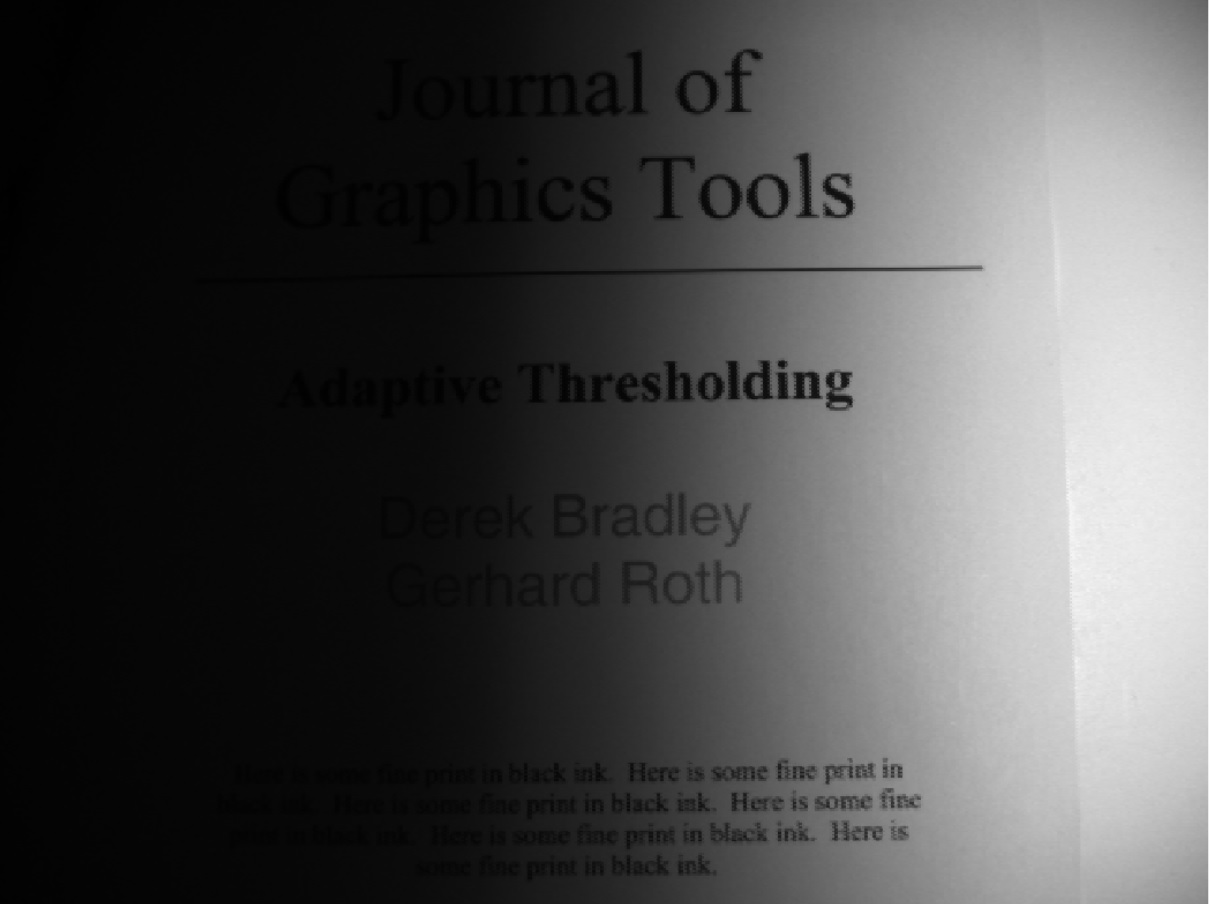
\includegraphics[width=0.28\textwidth]{graphics/paper_sample_2_input.jpg}}
    \subfigure[Output 2, Bradley's implementation \cite{Bradley2007}]{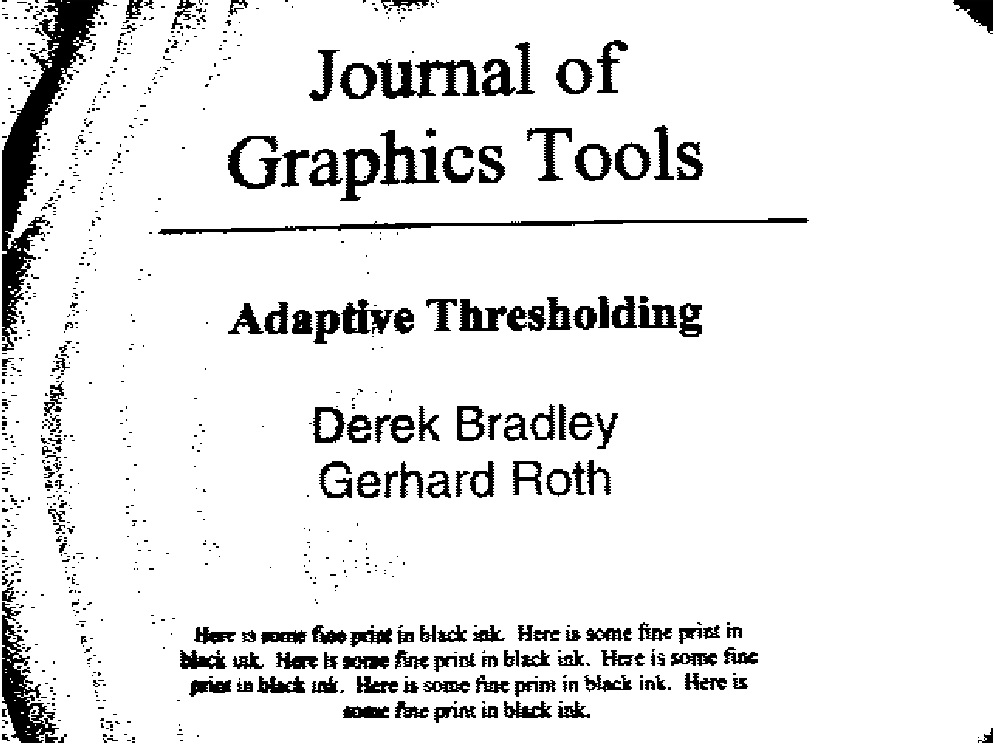
\includegraphics[width=0.28\textwidth]{graphics/sample_2_competitor.jpg}}
    \subfigure[Output 2, our implementation (n=80 w=35)]{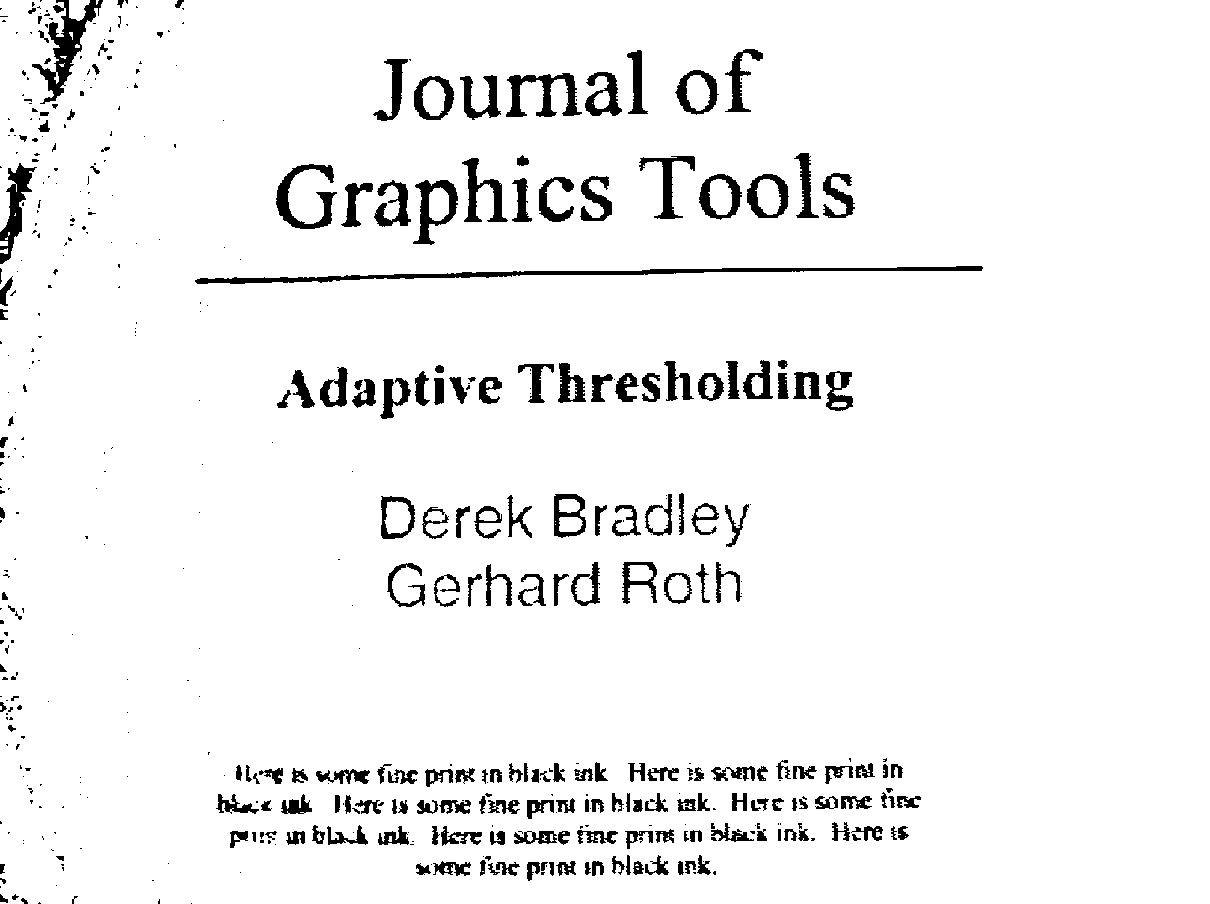
\includegraphics[width=0.28\textwidth]{graphics/paper_sample_2_output.jpg}} \\
    \caption{A comparison to Bradley's implementation \cite{Bataineh2011}}
    \label{fig*:comparison2}
\end{figure*}

\begin{figure*}
    \subfigure[Image 3]{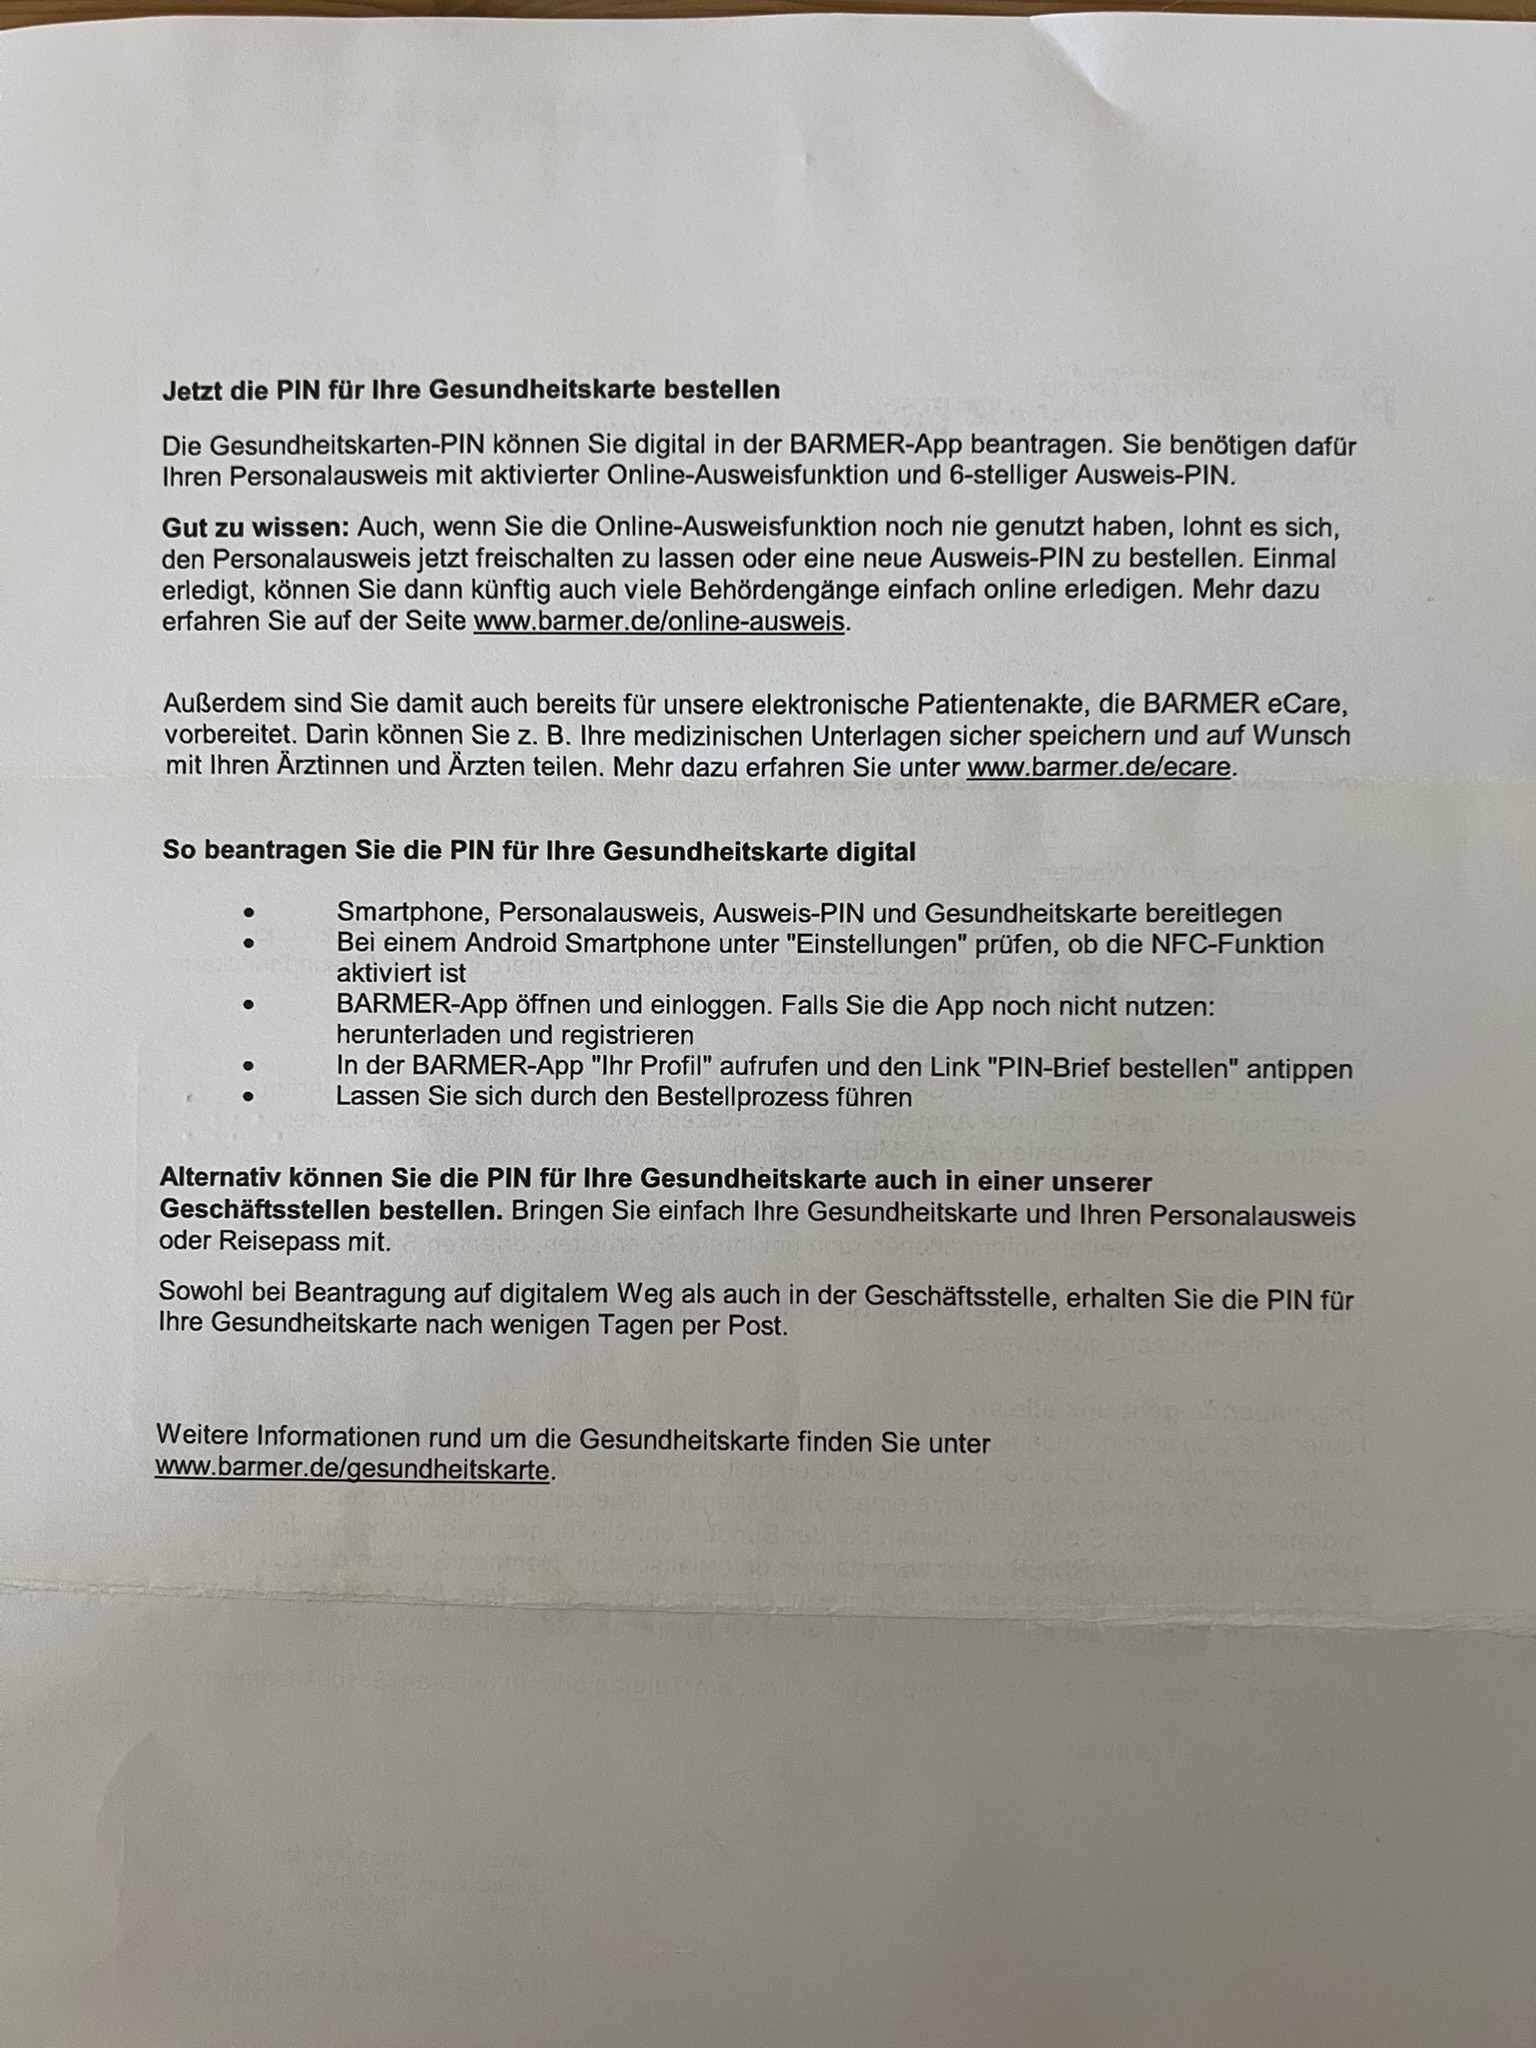
\includegraphics[width=0.28\textwidth]{graphics/paper_sample_3_input.jpg}}
    \subfigure[Output 3, our implementation (default parameters)]{
\includegraphics[width=0.28\textwidth]{graphics/paper_sample_3_output.jpg}} \\
    \caption{A real-world example. }
    \label{fig*:comparison3}
\end{figure*}


\subsection{Runtime Comparison}
Tables~\ref{tab:results1} and~\ref{tab:results2} shows the performance difference of the serial and parallel algorithm based on images 2 and 3, as they have different resolutions. Multiple window sizes were chosen to benchmark, as an increase in window size leads to an exponential increase in computational work. Luckily, in everyday scenarios, e.g. enhancing a picture of a printed email, window sizes can be chosen as small as 10-15.  
To measure the serial speed the program was executed with the \texttt{-s} flag, ensuring that only the computational power of one thread is being used.

All measurements were taken with the \texttt{-b} benchmarking flag under the same conditions, and the laptop was being charged at all times, making sure that no throttling was present. In both tables~\ref{tab:results1} and~\ref{tab:results2}, we can see a runtime speedup of up to \texttt{11x} on the desktop computer, while the laptop gets a maximum speedup of \texttt{8x} compared to the serial version.\newline 

On both machines, we can observe a trend that the lowest window size benchmarked has the least speedup of \texttt{8x} for desktop and \texttt{4x} for laptop. These diminishing returns are likely caused by the parallelization overhead slowly outweighing the speedup of parallelized work for smaller workloads. 

\begin{table}[htbp]
  \caption{Comparison of the running times and speedup of the image enhancement algorithm based on two pictures and three different window sizes per picture. Measurements were taken on a
desktop pc running Windows 10 Version 22H2 running on an AMD Ryzen 7 5800X (8 cores, 16 threads) CPU.}
  \label{tab:results1}
\resizebox{\columnwidth}{!}{
    \begin{tabular}{lcccrr}
      \toprule
      Image   & Resolution  & Window Size & Serial (s) & Parallel (s) & Speedup \\
      \midrule
      \multirow{3}{*}{Image\_2} & \multirow{3}{*}{1210×904} 
      & 20  & 0.455 & 0.056 & \textbf{8.07} \\
      &  & 50  & 2.703 & 0.249 & \textbf{10.84} \\
      &  & 100 & 0.916 & 1.031 & \textbf{10.59} \\
      \midrule
      \multirow{3}{*}{Image\_3} & \multirow{3}{*}{1536×2048}  
      & 20  & 1.328 & 0.152 & \textbf{8.75} \\
      &  & 50  & 7.814 & 0.71 \textbf{11.01} \\
      &  & 100 & 31.977 & 3.038 & \textbf{10.53} \\
      \bottomrule
    \end{tabular}
}
\end{table}


\begin{table}[htbp]
  \caption{Comparison of the running times and speedup of the image enhancement algorithm based on two pictures and three different window sizes per picture. Measurements were taken on a
laptop running Windows 11 Version 24H2 running on an Intel Core i5-12500H (12 cores, 16 threads) CPU.}
  \label{tab:results2}
\resizebox{\columnwidth}{!}{
    \begin{tabular}{lcccrr}
      \toprule
      Image   & Resolution  & Window Size & Serial (s) & Parallel (s) & Speedup \\
      \midrule
      \multirow{3}{*}{Image\_2} & \multirow{3}{*}{1210×904} 
      & 20  & 0.349 & 0.087 & \textbf{3.99} \\
      &  & 50  & 1.969 & 0.249 & \textbf{7.9} \\
      &  & 100 & 7.5 & 1.363 & \textbf{5.5} \\
      \midrule
      \multirow{3}{*}{Image\_3} & \multirow{3}{*}{1536×2048}  
      & 20  & 1.044 & 0.201 & \textbf{5.19} \\
      &  & 50  & 5.969 & 0.984 & \textbf{6.07} \\
      &  & 100 & 22.801 & 3.635 & \textbf{6.27} \\
      \bottomrule
    \end{tabular}
}
\end{table}

\section{Conclusions}
Based on the runtime benchmark results, the time needed to enhance even a high resolution picture seems reasonable. This is further amplified by the fact that in real-world scenarios, the window size can often be chosen as low as 10-15 without implications. Therefore, the overall image enhancement project can be seen as a success.

\subsection{Future Work}
A considerable amount of time has been spent researching about ways to measure the noise level of an image, with the end goal of finding a way to implement an automatic estimation for the best noise multiplier and window size parameters per picture. While there are multiple methods to compute an estimation of such noise level, a solution has yet not yet been found to either:
\begin{enumerate}
    \item approximate good parameters or
    \item automatically try out different parameters until a good noise level is reached.
\end{enumerate}
While the second option seems easy, it is easier said than done as all pictures have different preferred noise levels for optimal enhancement. If further work were to be done on this project, the main goal would be to find correlations between image parameters like mean color, standard deviation, min deviation and max deviation in combination with the preferred noise levels for maximum enhancement. A further approach would be to train a machine learning model to estimate noise levels at which an image would look the best.

%%
%% The next two lines define the bibliography style to be used, and
%% the bibliography file.
\bibliographystyle{ACM-Reference-Format}
\bibliography{literature}


\end{document}
\endinput
%%
%% End of file `sample-sigconf.tex'.
